file:///home/ql/5/AA/report/1/3-design.tex {"mtime":1601728718495,"ctime":1600807997322,"size":1824,"etag":"35omieodk1rq","orphaned":false}
\chapter{Конструкторский раздел}
\label{cha:design}

В данном разделе будет приведено описание схем алгоритмов
нахождения расстояния Левенштейна и Дамерау-Левенштейна

\section{Разработка алгоритмов}
% схемы алгоритмов

На рисунках показаны схемы алгоритмов Левенштейна
рекурсивная, матричная, рекурсивная реализация с заполнением матрицы
и схема алгоритма Дамерау–Левенштейна (матричная).

Примечание: я создаю таблицы и инициализирую значение вне этих функции


\pagebreak
\subsection{Схема алгоритма Левенштейна}

\begin{figure}[h]
    \centering
    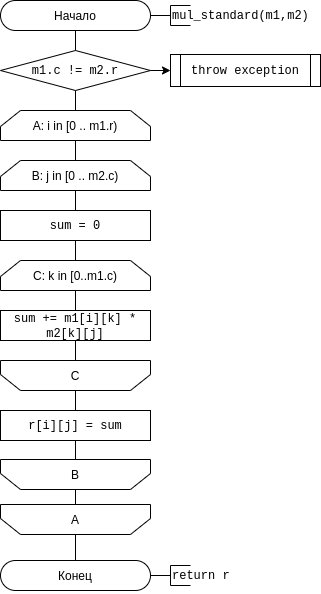
\includegraphics[width=0.7\textwidth]{1/inc/d1.png}
    \caption{Схема рекурсивного алгоритма Левенштейна}
\end{figure}

\pagebreak
\begin{figure}[h]
    \centering
    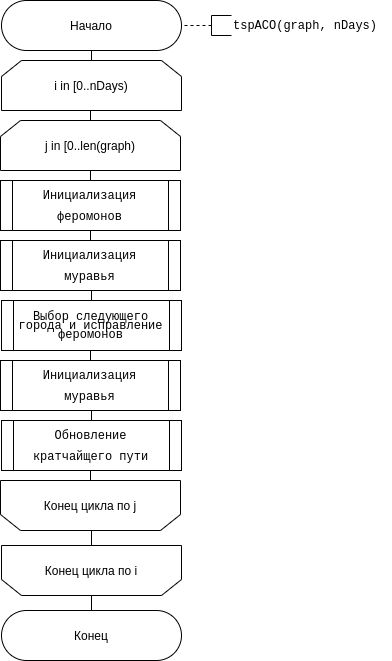
\includegraphics[width=0.65\textwidth]{1/inc/d2.png}
    \caption{Схема матричного алгоритма Левенштейна}
\end{figure}

\pagebreak
\begin{figure}[h]
    \centering
    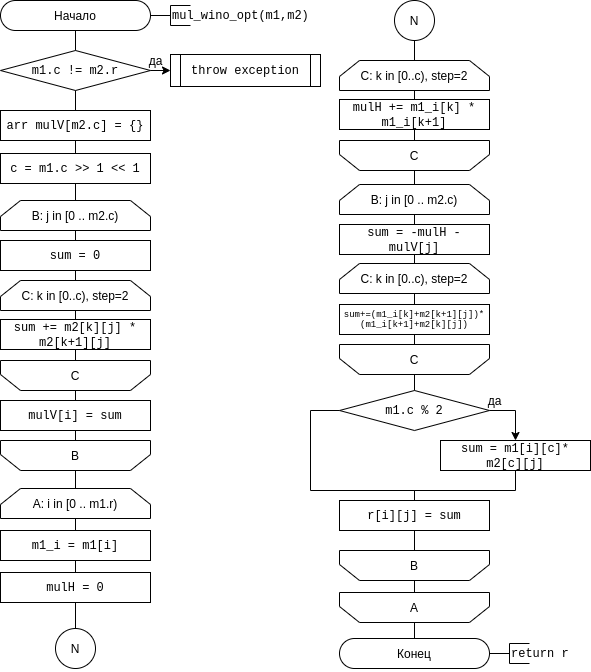
\includegraphics[width=0.8\textwidth]{1/inc/d3.png}
    \caption{Схема мемоизационного алгоритма Левенштейна}
\end{figure}


\newpage
\subsection{Схема алгоритма Дамерау — Левенштейна}

\begin{figure}[]
    \centering
    \includegraphics[width=0.65\textwidth]{1/inc/d4.png}
    \caption{Схема матричного алгоритма Дамерау — Левенштейна}
\end{figure}